\begin{figure}[H]
  \centering
  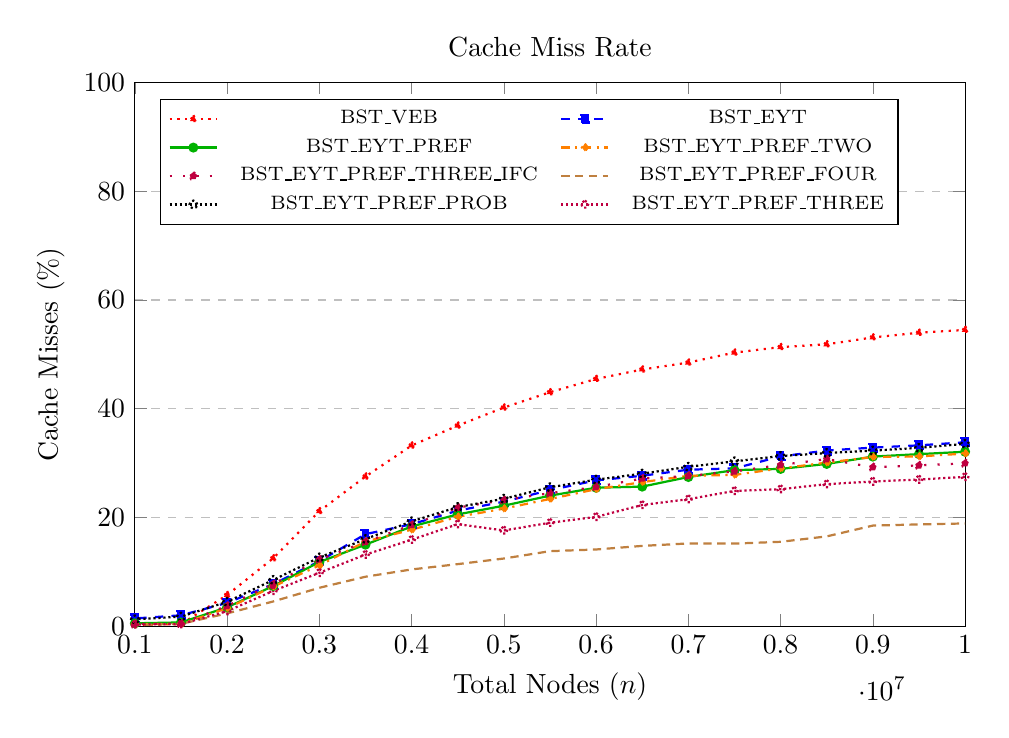
\begin{tikzpicture}
    \begin{axis}[
        title={Cache Miss Rate},
        xlabel={Total Nodes ($n$)},
        ylabel={Cache Misses (\%)},
        width=\textwidth,
        height=0.7\textwidth,
        xmin=1000000, xmax=10000000,
        ymin=0, ymax=100,
        ymajorgrids,
        grid style=dashed,
        legend columns=2,
        legend pos=north west,
        legend style={font=\scriptsize, column sep=6pt},
    ]

\addplot+[red, thick, dotted, mark=triangle*, mark options={scale=.7,fill=red}]
  coordinates {
    (500000,0.278984)
    (1000000,0.240263)
    (1500000,0.407462)
    (2000000,5.74785)
    (2500000,12.5086)
    (3000000,21.1631)
    (3500000,27.5335)
    (4000000,33.2375)
    (4500000,36.9037)
    (5000000,40.2233)
    (5500000,43.0436)
    (6000000,45.4827)
    (6500000,47.2207)
    (7000000,48.4906)
    (7500000,50.3293)
    (8000000,51.3401)
    (8500000,51.8523)
    (9000000,53.1175)
    (9500000,53.9807)
    (10000000,54.5)
  };
\addlegendentry{BST\_VEB}

\addplot+[blue, thick, dashed, mark=square*, mark options={scale=.7,fill=blue}]
  coordinates {
    (500000,0.683896)
    (1000000,1.43965)
    (1500000,2.02308)
    (2000000,4.30151)
    (2500000,7.74719)
    (3000000,11.9664)
    (3500000,16.9416)
    (4000000,18.7676)
    (4500000,21.2633)
    (5000000,22.9219)
    (5500000,25.0461)
    (6000000,26.8263)
    (6500000,27.6832)
    (7000000,28.7966)
    (7500000,29.0349)
    (8000000,31.235)
    (8500000,32.3206)
    (9000000,32.8568)
    (9500000,33.2711)
    (10000000,33.8411)
  };
\addlegendentry{BST\_EYT}

\addplot+[green!70!black, thick, solid, mark=*, mark options={scale=.7,fill=green!70!black}]
  coordinates {
    (500000,0.557928)
    (1000000,0.551707)
    (1500000,0.710955)
    (2000000,3.49059)
    (2500000,7.40254)
    (3000000,11.8162)
    (3500000,15.0154)
    (4000000,18.3543)
    (4500000,20.5759)
    (5000000,22.1757)
    (5500000,24.0226)
    (6000000,25.477)
    (6500000,25.6833)
    (7000000,27.4489)
    (7500000,28.7174)
    (8000000,28.9403)
    (8500000,29.8563)
    (9000000,31.2042)
    (9500000,31.6618)
    (10000000,32.0926)
  };
\addlegendentry{BST\_EYT\_PREF}

\addplot+[orange, thick, dashdotted, mark=diamond*, mark options={scale=.7,fill=orange}]
  coordinates {
    (500000,0.465832)
    (1000000,0.423322)
    (1500000,0.436638)
    (2000000,3.32215)
    (2500000,7.30333)
    (3000000,11.1973)
    (3500000,15.5859)
    (4000000,17.7575)
    (4500000,20.1276)
    (5000000,21.6356)
    (5500000,23.4139)
    (6000000,25.2078)
    (6500000,26.5085)
    (7000000,27.6708)
    (7500000,27.842)
    (8000000,29.0355)
    (8500000,30.0975)
    (9000000,31.1261)
    (9500000,31.2254)
    (10000000,31.7667)
  };
\addlegendentry{BST\_EYT\_PREF\_TWO}

\addplot+[purple, thick, loosely dotted, mark=pentagon*, mark options={scale=.7,fill=purple}]
  coordinates {
    (500000,0.41073)
    (1000000,0.396111)
    (1500000,0.467047)
    (2000000,3.75864)
    (2500000,7.77908)
    (3000000,12.2831)
    (3500000,15.5118)
    (4000000,18.6288)
    (4500000,21.82)
    (5000000,23.2005)
    (5500000,24.4833)
    (6000000,25.6155)
    (6500000,27.1685)
    (7000000,27.654)
    (7500000,28.4796)
    (8000000,29.6705)
    (8500000,30.7406)
    (9000000,29.2564)
    (9500000,29.5879)
    (10000000,29.9707)
  };
\addlegendentry{BST\_EYT\_PREF\_THREE\_IFC}

\addplot+[brown, thick, densely dashed, mark=x*, mark options={scale=.7,fill=brown}]
  coordinates {
    (500000,0.202168)
    (1000000,0.200024)
    (1500000,0.454122)
    (2000000,2.36806)
    (2500000,4.56377)
    (3000000,7.07849)
    (3500000,9.11493)
    (4000000,10.4538)
    (4500000,11.4291)
    (5000000,12.4623)
    (5500000,13.8118)
    (6000000,14.1229)
    (6500000,14.7818)
    (7000000,15.2367)
    (7500000,15.2066)
    (8000000,15.5347)
    (8500000,16.5298)
    (9000000,18.5165)
    (9500000,18.7363)
    (10000000,18.9125)
  };
\addlegendentry{BST\_EYT\_PREF\_FOUR}

\addplot+[black, thick, densely dotted, mark=o, mark options={scale=.7,fill=black}]
  coordinates {
    (500000,0.696147)
    (1000000,1.27225)
    (1500000,1.77507)
    (2000000,4.50111)
    (2500000,8.51703)
    (3000000,12.6561)
    (3500000,16.0357)
    (4000000,19.289)
    (4500000,21.9189)
    (5000000,23.4505)
    (5500000,25.5584)
    (6000000,26.9603)
    (6500000,28.0666)
    (7000000,29.3306)
    (7500000,30.3312)
    (8000000,31.3106)
    (8500000,31.8534)
    (9000000,32.2998)
    (9500000,32.8115)
    (10000000,33.5532)
  };
\addlegendentry{BST\_EYT\_PREF\_PROB}

\addplot+[purple, thick, densely dotted, mark=pentagon, mark options={scale=.7,fill=purple}]
  coordinates {
    (500000,0.301372)
    (1000000,0.334791)
    (1500000,0.405097)
    (2000000,2.77965)
    (2500000,6.49974)
    (3000000,9.83752)
    (3500000,13.1832)
    (4000000,15.9192)
    (4500000,18.7819)
    (5000000,17.6228)
    (5500000,19.0392)
    (6000000,20.1172)
    (6500000,22.3047)
    (7000000,23.3728)
    (7500000,24.8941)
    (8000000,25.2068)
    (8500000,26.1395)
    (9000000,26.6233)
    (9500000,26.99)
    (10000000,27.4763)
  };
\addlegendentry{BST\_EYT\_PREF\_THREE}
    \end{axis}
  \end{tikzpicture}
  \caption[Total Cache Miss Rate of different Implementations]{Total Cache miss rate (\%) as a function of total nodes and lookups ($q=1000000$) for the different implementations. A miss in this case means we have to load the value from main memory.}
  \label{fig:cachemissbig}
\end{figure}
